El simulador VREP es una plataforma de control distribuido a traves de diferentes plataformas y lenguajes de programaci\'on que provee a los desarrolladores de herramientas vers\'atiles para las aplicaciones multi-robots. Los controadores pueden ser escritos en C/C++, Python, Java, Lua, Matlab, Octave o Urbi. \\

Antes de la implementaci\'on sobre dispositivos reales, de cara a probar la efectividad del algoritmo, se han realizado una serie de pruebas y simulaciones descritas en el siguiente cap\'itulo. 

\subsection{Interfaz de Usuario Gr\'afica}

La siguiente imagen \ref{fig:VREP_GUI} muestra la interfaz t\'ipica de la aplicaci\'on. Algunos objetos preprogramados pueden encontrarse en el menu de la izquierda (Desde robots m\'oviles hasta material de atrezo para dotar de realismo a las simulaciones)

\begin{figure}
	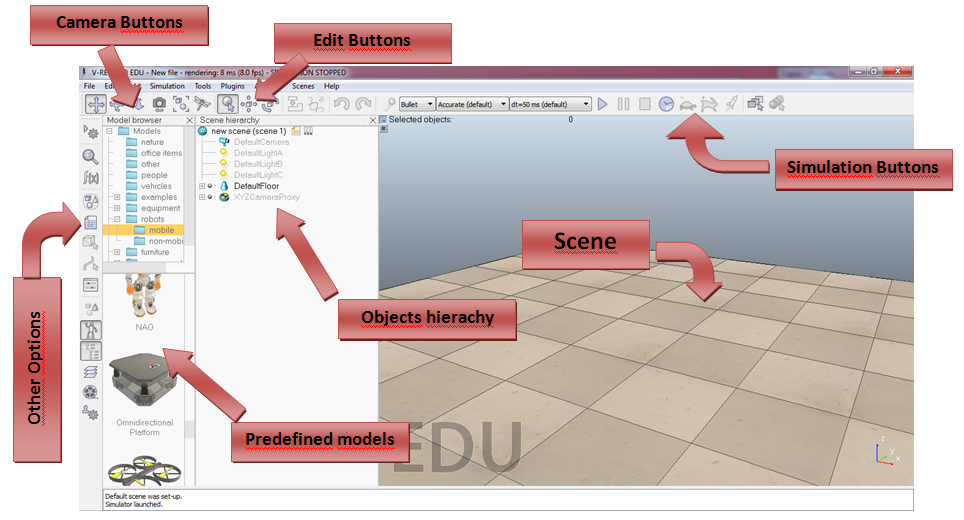
\includegraphics[width=\textwidth,natwidth=964,natheight=520]{../Images/c3/vrep_main.png}
	\caption{V-REP GUI}
	\label{fig:VREP_GUI}
\end{figure}


